%EKG-7 Android-App
\subsection{Android-App}
Dieses Unterkapitel behandelt den Entwurf und die Entwicklung der Home-EKG Android App zur Darstellung eines EKG Signals unter Verwendung der Bluetooth 2.0 Technologie. Die Kommunikation mit einer Datenbank ermöglicht es in Echtzeit Patientendaten zu speichern, sowie Authentifizierungsabfragen durchzuführen. Das Projekt wurde hauptsächlich mit der objektorientierten Programmiersprache Java realisiert. 

\subsubsection{Datenbank}
Um eine geräteübergreifende Funktionalität aller Features der Android App zu gewährleisten wurde bei der Entwicklung auf die Echtzeitdatenbank \textit{Firebase} \cite{Firebase}  zurückgegriffen. Die von Google bereitgestellte IDE Android Studio \cite{Android_Studio} ermöglicht eine besonders einfache Implementierung der verschiedenen Funktionalitäten der Datenbank wie Authentifizierung und Cloud-Speicherung. \\
Bei der Registrierung eines Anwenders wird ein neuer \textit{Child-Node} im Benutzer-Baum angelegt und mit einer individuellen Identifikationsnummer ausgestattet. Über diese kann die App mit dem Server kommunizieren und Daten austauschen. \\
Der Benutzer hat außerdem die Möglichkeit ein Profilbild im .png Format hochzuladen, welches in einen von \textit{Firebase} verwalteten externen Speicher abgelegt wird. Durch die Verwendung von Google Analytics \cite{Google_Analytics} kann ferner das Nutzerverhalten statistisch erfasst und auf verschiedene Arten ausgewertet werden. 

\subsubsection{Aktivitäten}

\begin{wrapfigure}[12]{R}{0.4\textwidth}
\vspace{-25pt}
\includegraphics[width=0.4\textwidth]{app_Activity.png}
\caption{Lebenszyklus}
\label{app_Activity}
\end{wrapfigure}

Jede \textit{Activity}-Klasse \cite{Activity_Overview} stellt einen Bildschirm (Login Seite, Register Seite oder Profil Seite) der App dar, mit welcher der Benutzer interagieren und somit Befehle an das Betriebssystem weitergeben kann. Beim Start einer neuen Aktivität wird eine Instanz der zugrunde liegenden Java Klasse erzeugt und der zugehörige Lebenszyklus (Abbildung \ref{app_Activity}) gestartet. \cite{Activity_Lifecycle}
Um zwischen den drei Hauptzuständen

\begin{itemize}
	\item[•] Aktivität läuft im Vordergrund und hat Fokus
	\item[•] Aktivität läuft im Hintergrund
	\item[•] Aktivität wurde gestoppt
\end{itemize}

zu wechseln, bietet die \textit{Activity} Klasse außerdem einen Satz von sechs \textit{Callback} an, die bei Übergängen von verschiedenen Phasen des Lebenszyklus aufgerufen werden. Durch Verwendung der \textit{onCreate()} Methode können so zum Beispiel Buttons oder Textfelder initialisiert werden.
Die Home-EKG App besteht insgesamt aus sieben Aktivitäten, welche im Folgenden einzeln vorgestellt werden.

\begin{itemize}
\item Login und Registrierung Aktivität: Die Login Aktivität (Abbildung \ref{app_login_reg} links) stellt den Einstieg des Benutzers in die App dar. Grundlegend werden drei Login Varianten angeboten, wobei der Benutzer nur bei der Methode über E-Mail einen neuen Account anlegen muss, bevor er die App verwenden kann. Die Implementierung der Services von Facebook und Google erlauben es dem Nutzer sich über bereits bestehende Accounts anzumelden, ohne eine erneute Registrierung vornehmen zu müssen. \\
Außerdem besteht die Möglichkeit durch Setzten des Hakens im Feld \textit{Remember me} die Daten für zukünftige Anmeldeversuche lokal in einem privaten \textit{SharedPreferences}-Objekt zu speichern, um beim nächsten Start der App die Login Seite zu überspringen und direkt zur Main Aktivität weitergeleitet zu werden. \\
Bei Betätigung des Login Buttons wird eine Verbindung zum Server der Datenbank aufgebaut und die in den zwei TextInput-Feldern eingegebenen Zeichen an Googles \textit{Firebase} geschickt. Bei erfolgreichem Abgleich werden die Benutzerdaten vom Server heruntergeladen und der Benutzer zum Main Screen weitergeleitet. \\
Durch einen Klick auf \textit{Register Now} oder Plus wird eine neue Registrierungs-Aktivität gestartet (Abbildung \ref{app_login_reg} rechts). Die Felder Name, Passwort und E-Mail sind verpflichtend auszufüllen. Durch Versenden einer Bestätigungs-Mail wird die Validität der Adresse überprüft und der Account erst nach erfolgreicher Bestätigung erstellt.
	\begin{figure} [!h]
		\begin{center}
			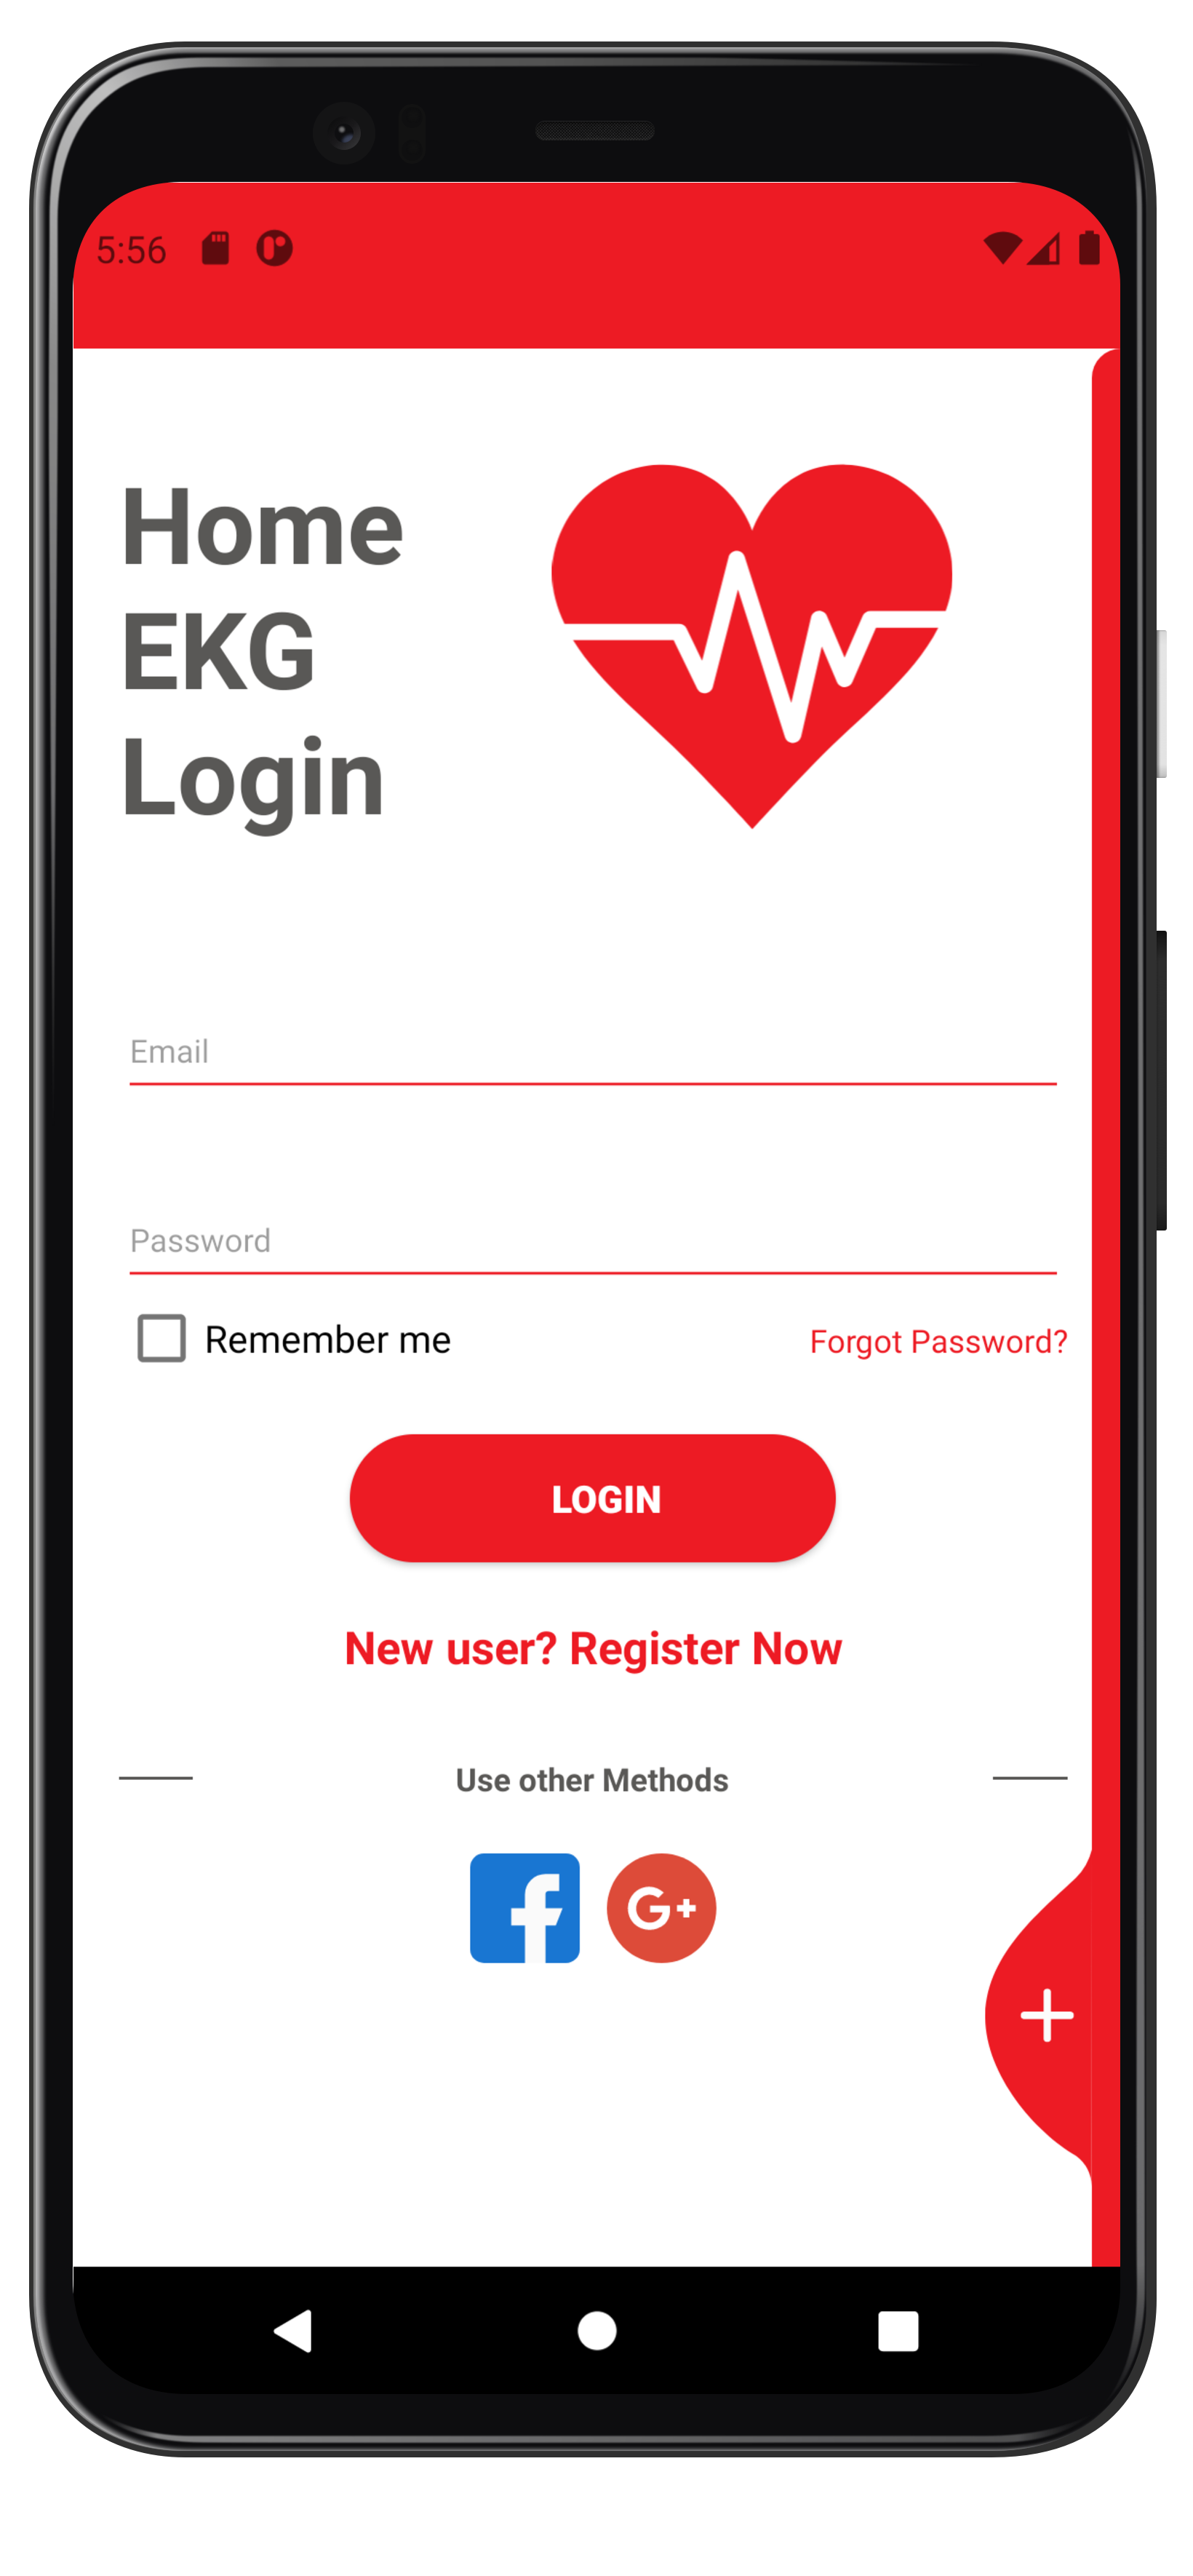
\includegraphics[width=150pt]{app_login.png}
			\hspace{1.5 cm}
			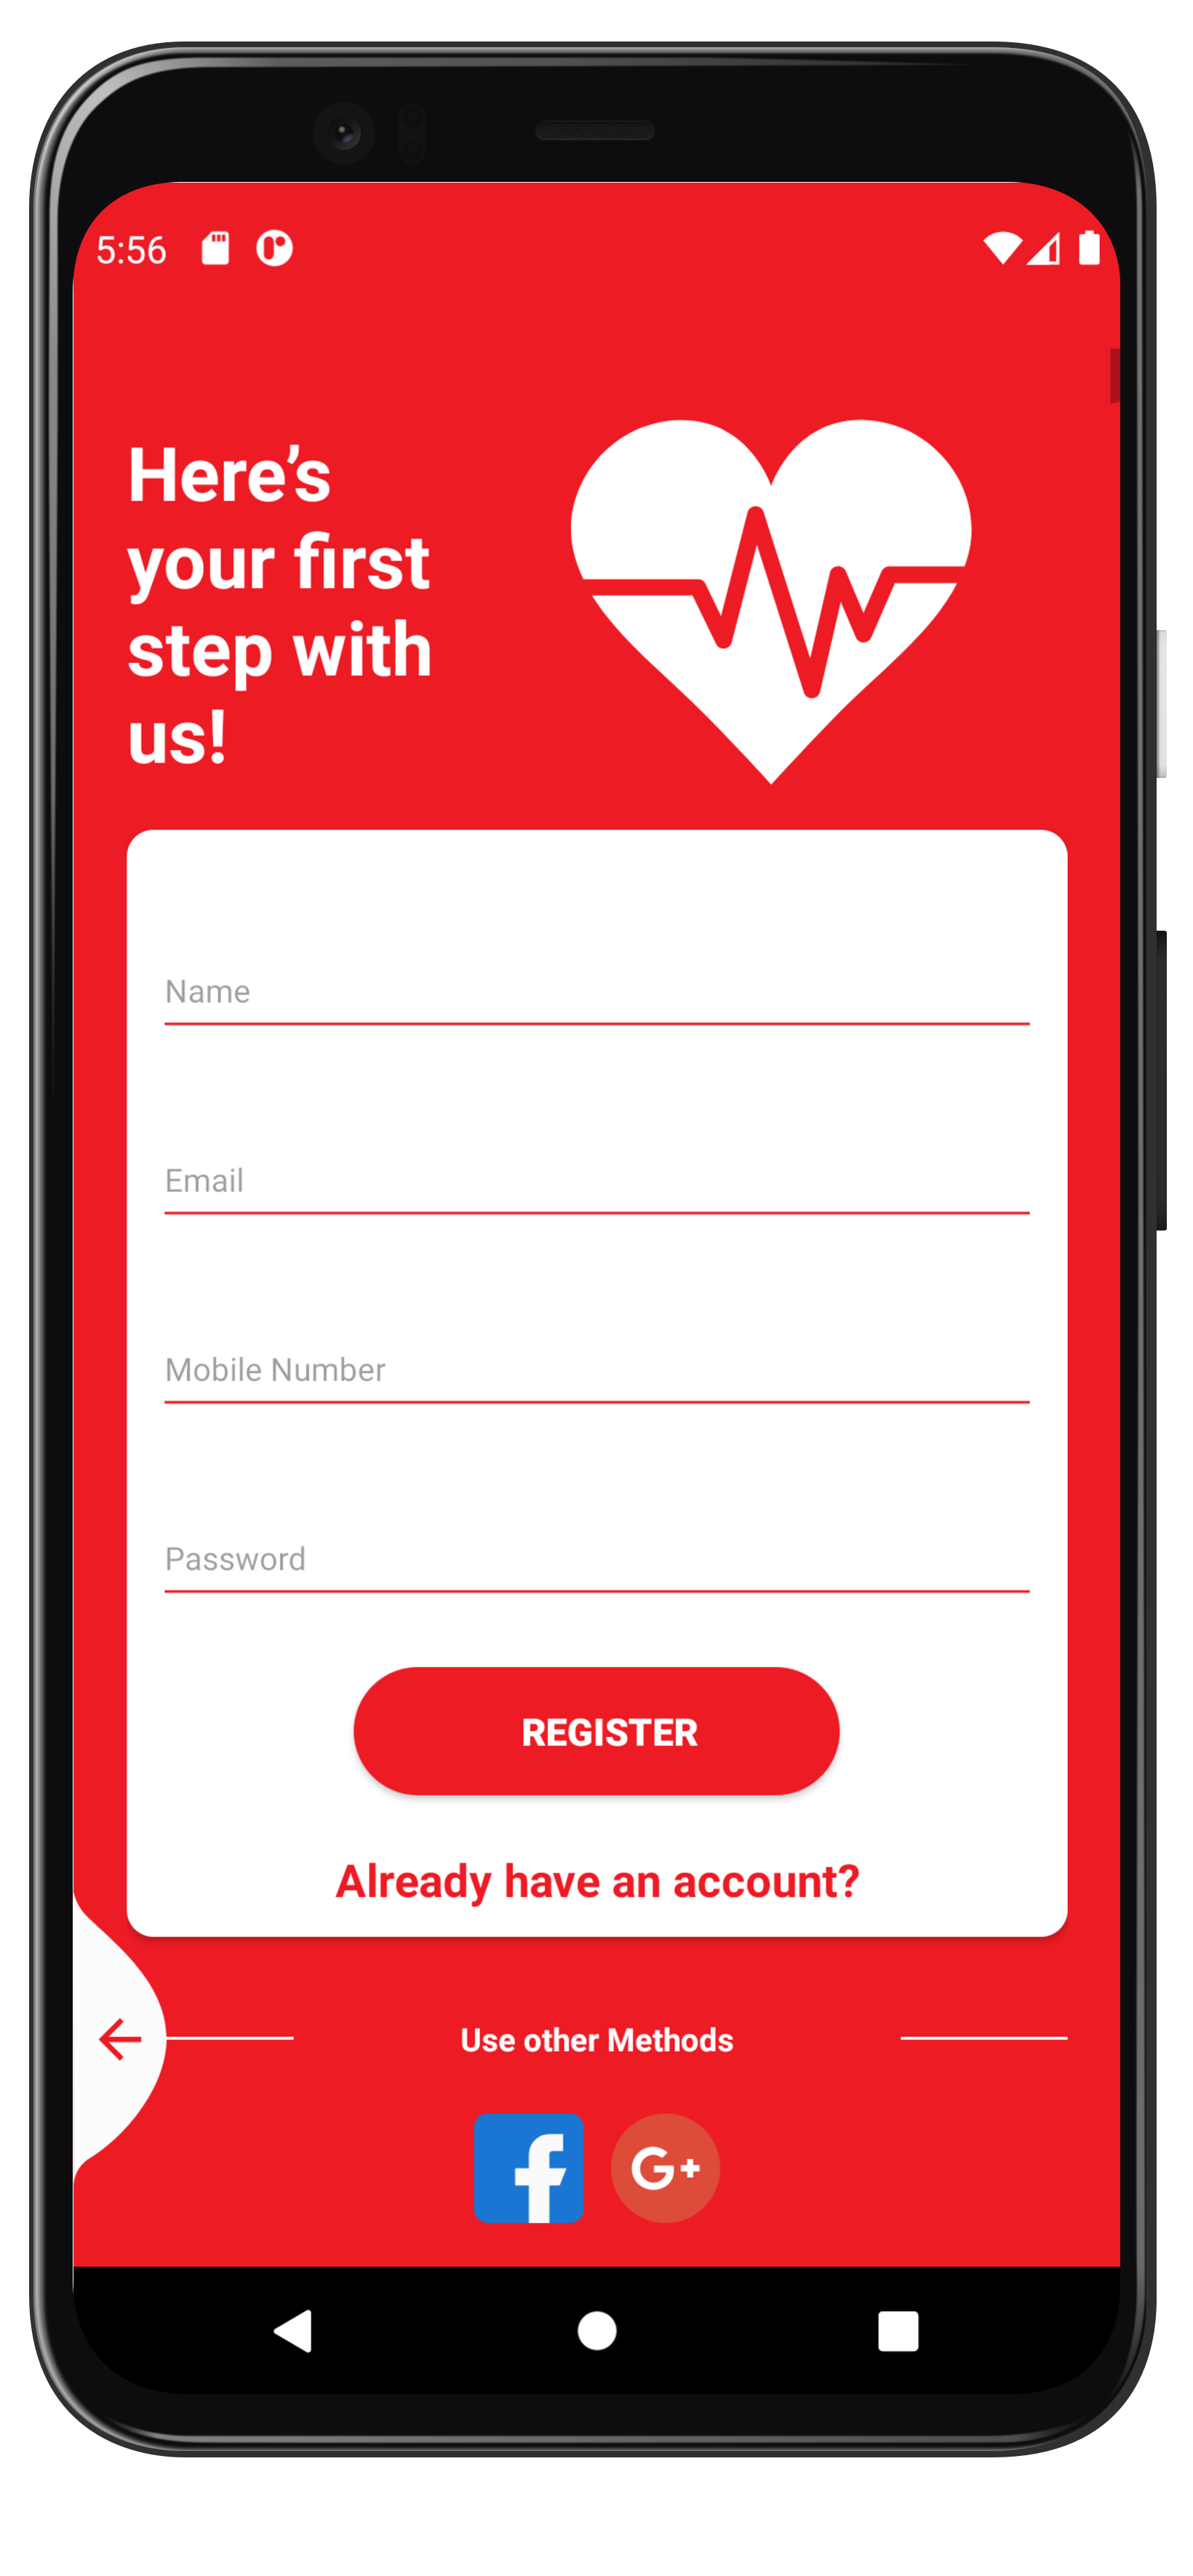
\includegraphics[width=150pt]{app_register.png}
		\end{center}
		\caption{Login und Registrierungs Aktivität}
		\label{app_login_reg}
	\end{figure}

\item Home Aktivität: Die Home Aktivität (Abbildung \ref{app_profile_scan} links) stellt dem Benutzer eine Schnittstelle zum Datenbank Server bereit, um seine Daten erstmalig hochzuladen und zu einem späterem Zeitpunkt aktualisieren zu können. Wird zum Beispiel das Gewicht verändert und eine Update Anfrage an \textit{Firebase} geschickt, wird auch nur dieser \textit{Child Node} der Benutzerreferenz aktualisiert und nicht das ganze Profil erneut hochgeladen. \\
Durch einen implementierten \textit{onDataChange()} Listener werden serverseitige Änderungen auch direkt in Echtzeit auf der Home Aktivität aktualisiert, ohne dabei eine ständige Verbindung halten zu müssen. Die folgenden Attribute sind personalisierbar: Mail, Geschlecht, Geburtsdatum, Größe, Gewicht, Wohnort und Versicherung.\\
Durch Drücken auf das Stift-Symbol unterhalb des Profilbildes, wird ein \textit{Action Intent} generiert, der die auf dem Smartphone als standardmäßige eingestellte Galerie öffnet und den Benutzer ein personalisiertes Profilbild auswählen lässt. Im \textit{onActivityResult()} Callback wird dem Foto eine URI zugeordnet und in den \textit{Firebase}-Speicher hochgeladen. Bei einem Login über ein anderes Gerät wird nun auch das neue Profilbild angezeigt und lokal im Speicher hinterlegt, um den Internetdatenverbrauch zu minimieren. \\
Über das Dropdown Menu in der oberen rechten Ecke kann der Benutzer einen Abmeldedialog starten, wobei auch die \textit{Shared Preferences}-Variable der Auto Login Checkbox zurückgesetzt wird. Der Button „Connect to EKG“ leitet den Benutzer zur Signal Aktivität weiter.
\begin{figure} [!h]
	\begin{center}
		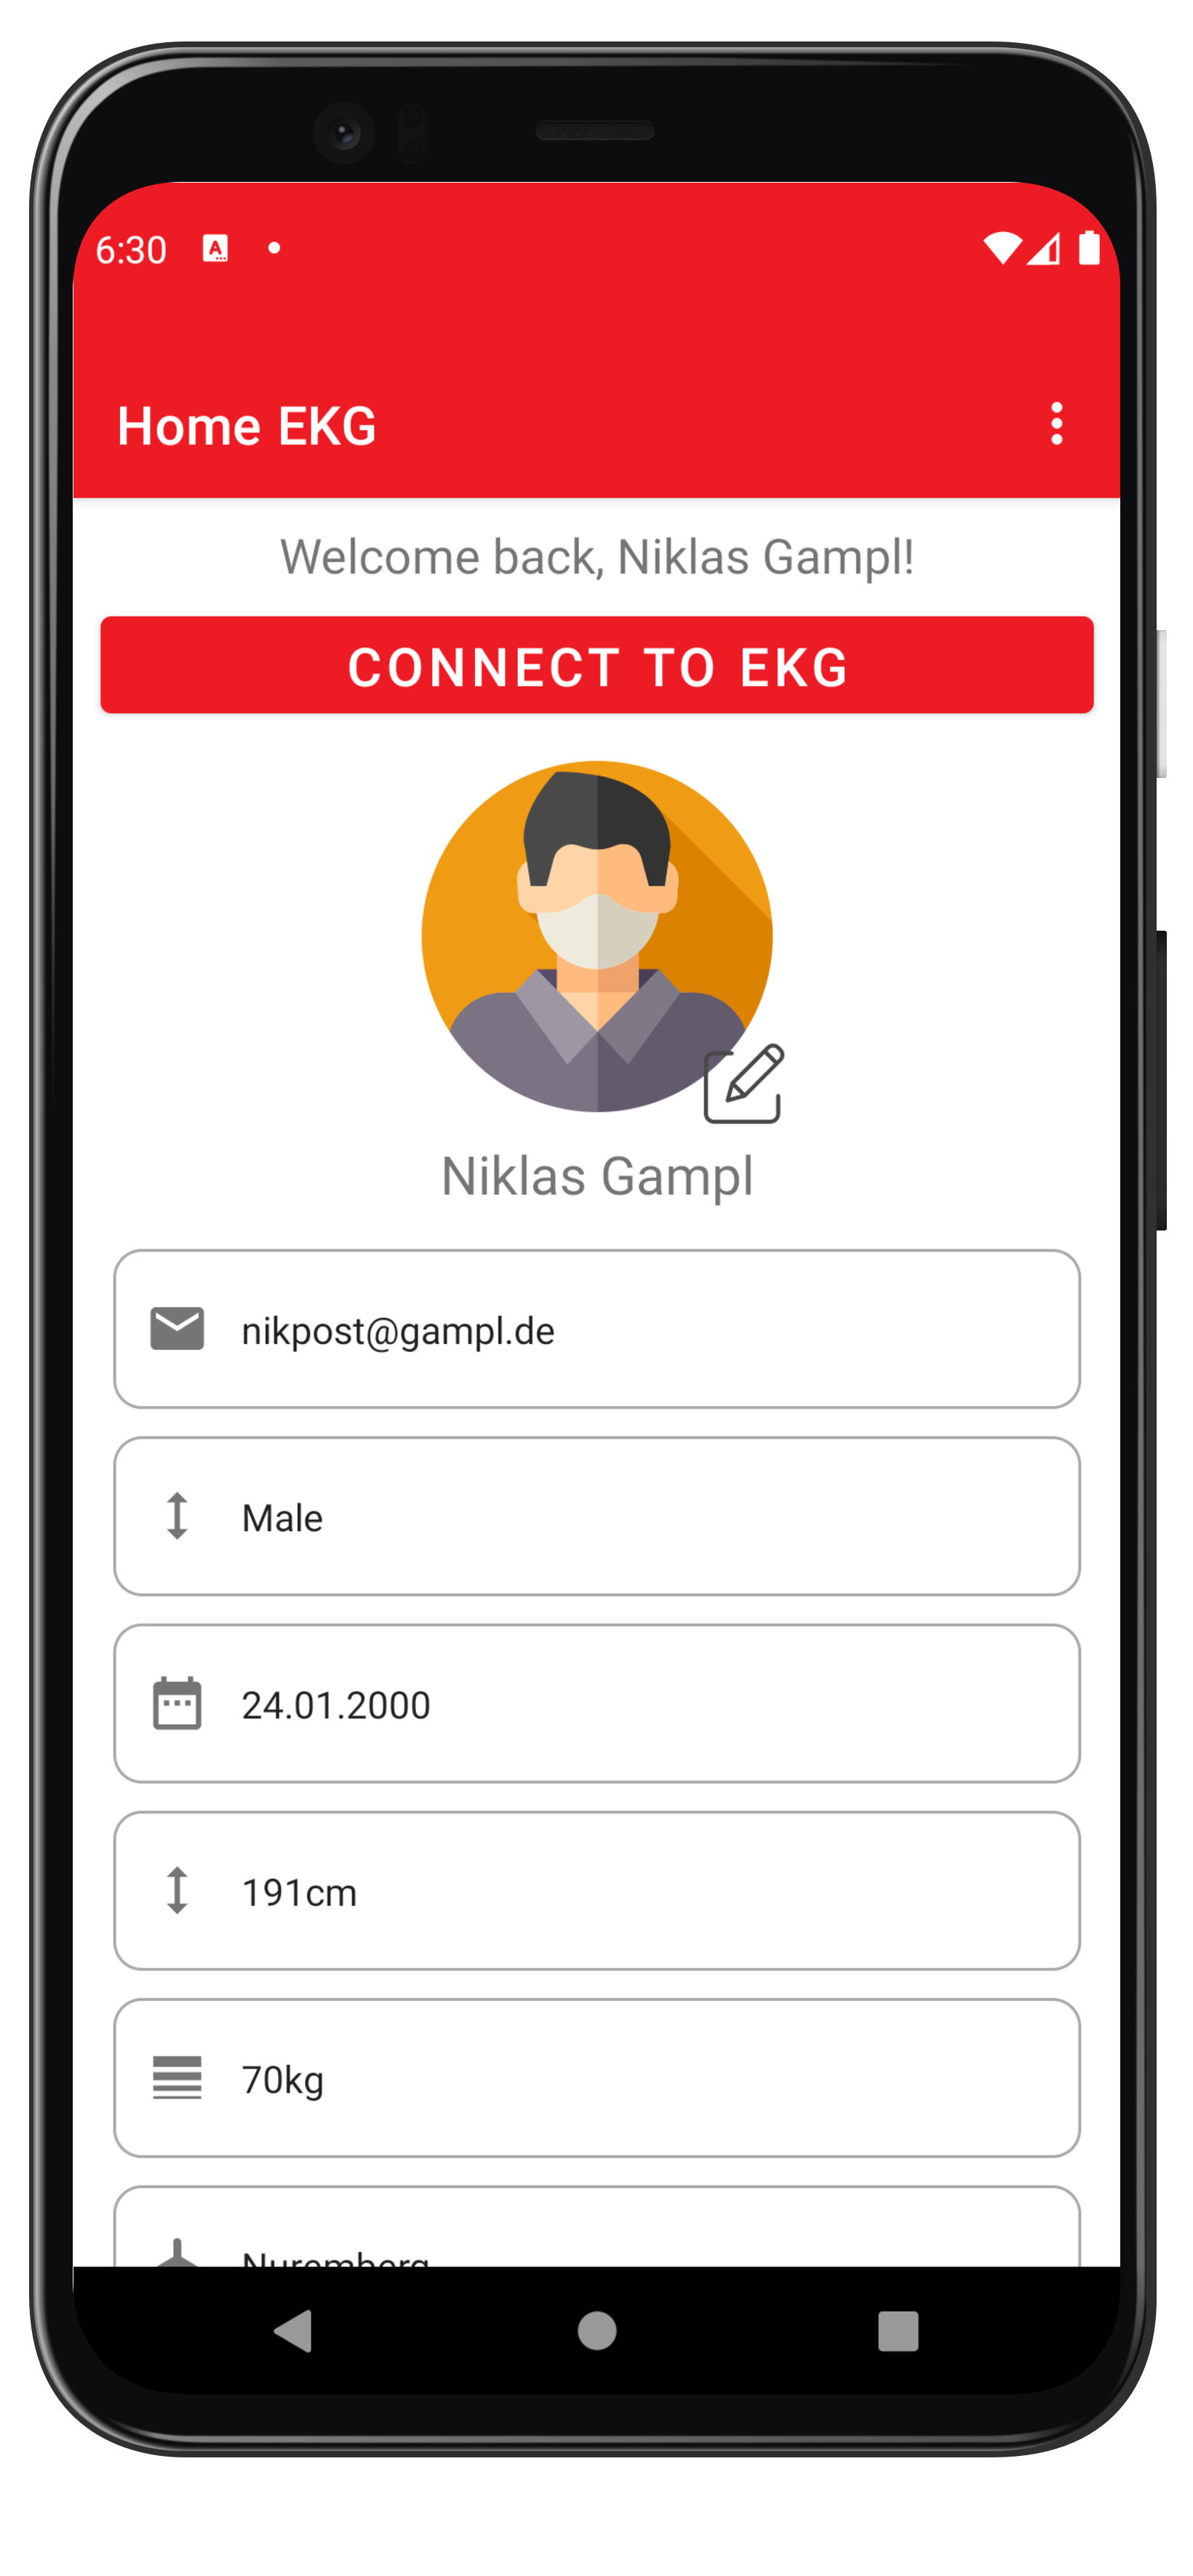
\includegraphics[width=150pt] {app_profile.png}
		\hspace{1.5 cm}
		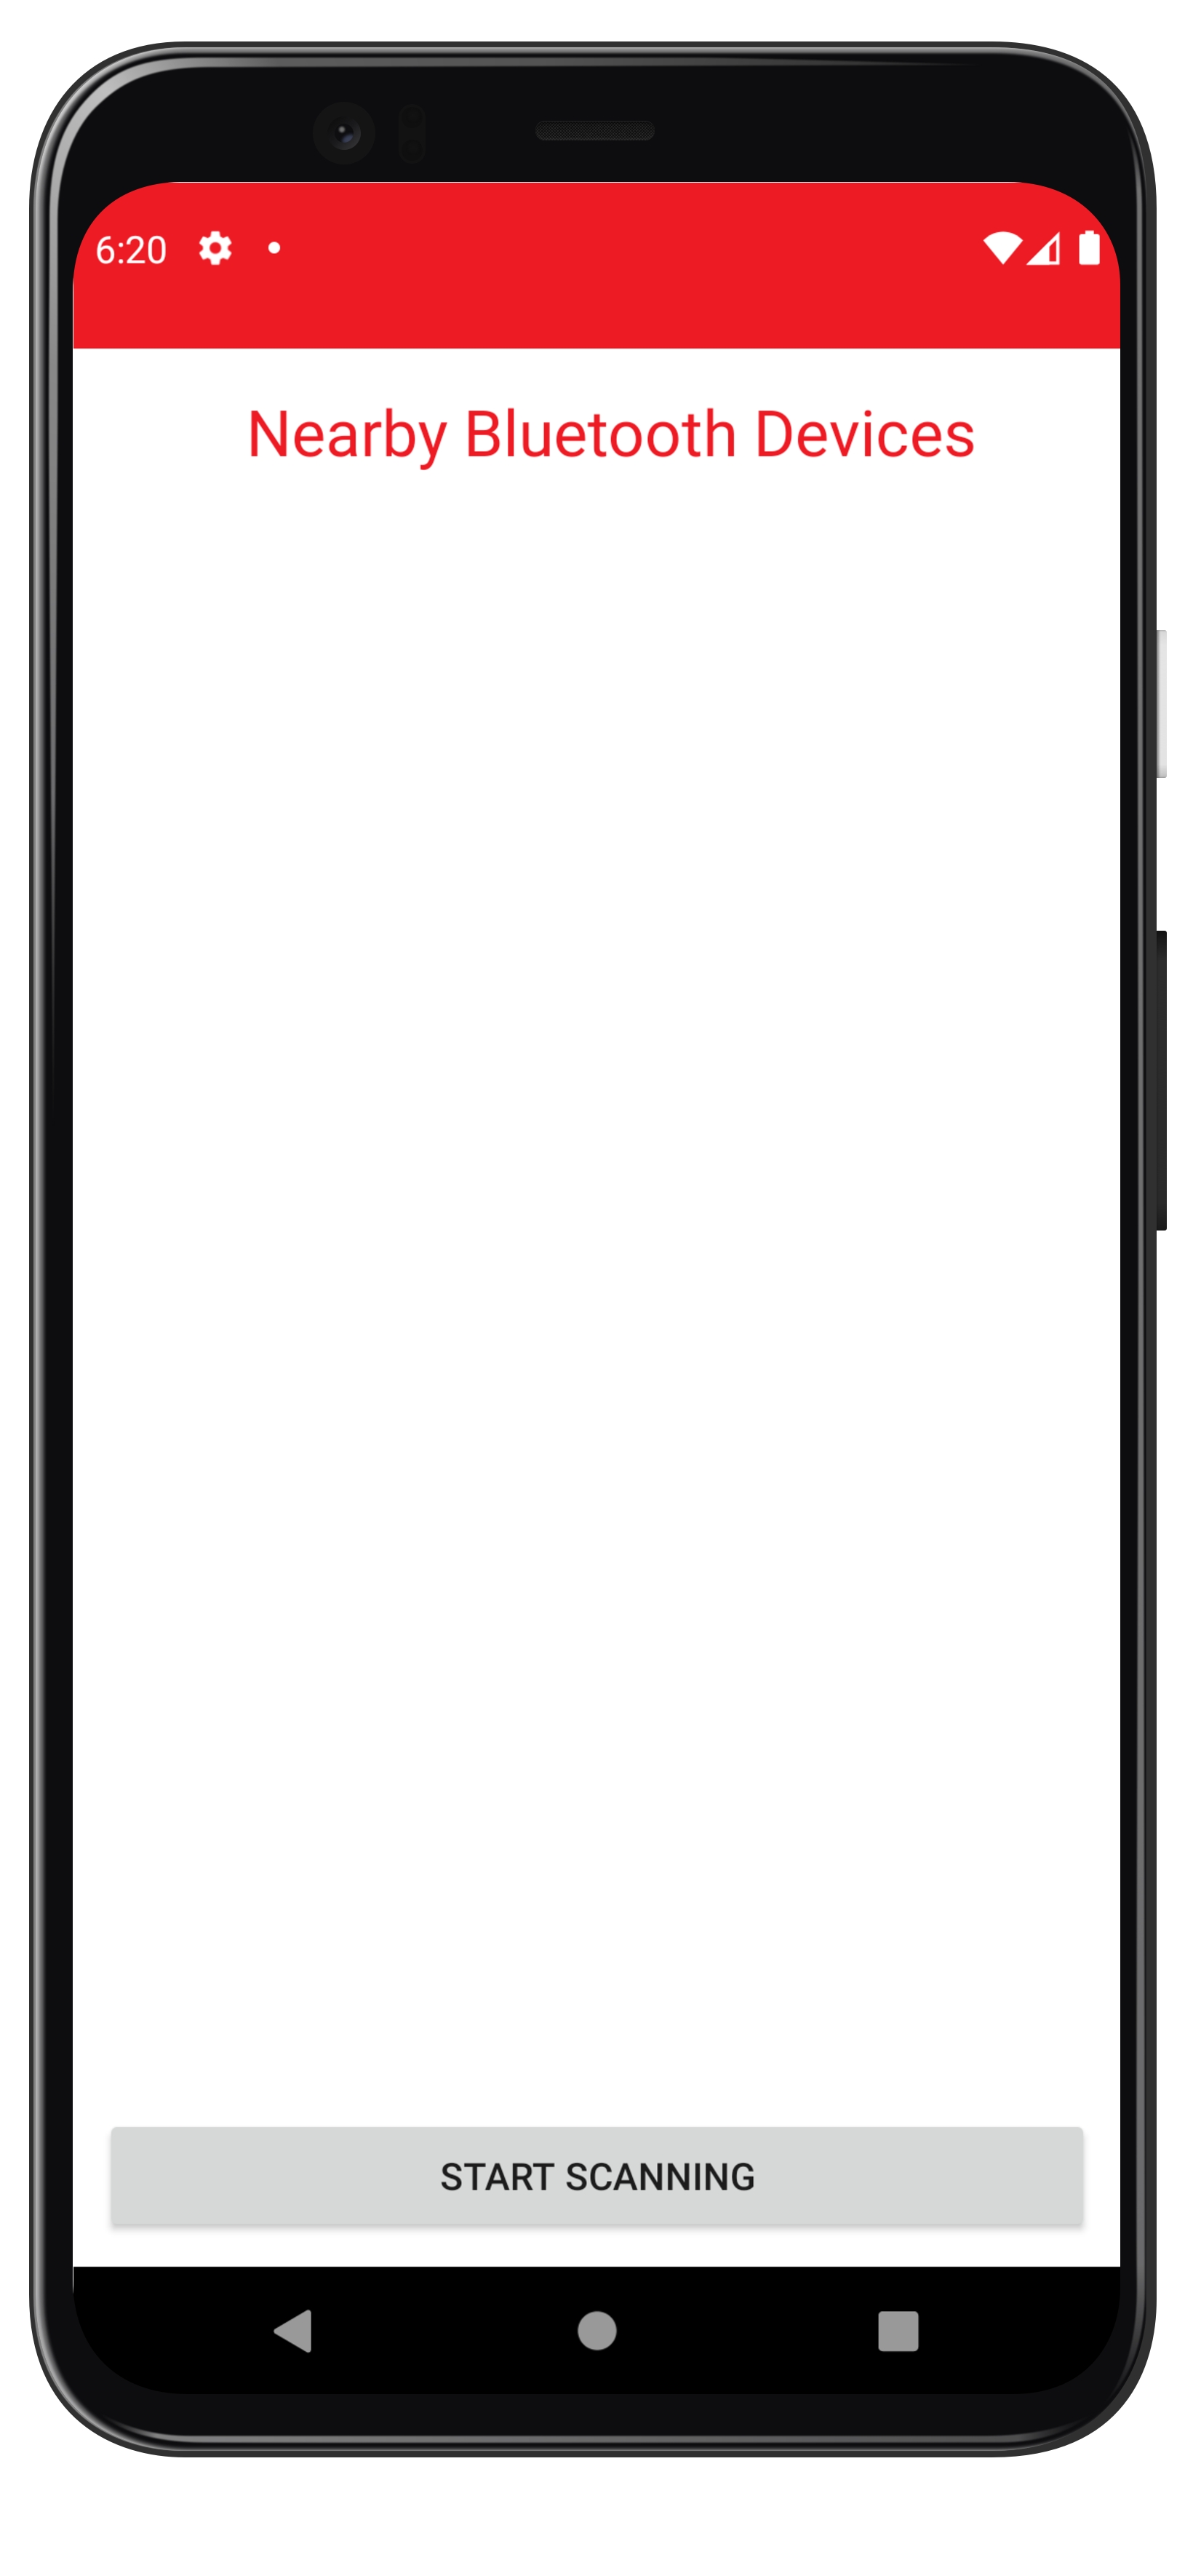
\includegraphics[width=150pt] {app_scan.png}
	\end{center}
	\caption{Profil und Scanner Aktivität}
	\label{app_profile_scan}
\end{figure}

\item Signal und Scanner Aktivität: Die Signal Aktivität (Abbildung \ref{app_signal}) stellt die Hauptfunktionalität der App, das Anzeigen eines Echtzeit EKG Signals, bereit. Durch Drücken auf den Connect Button wird der Benutzer zur Scanner Aktivität (Abbildung \ref{app_profile_scan} rechts) weitergeleitet und aufgefordert Bluetooth zu aktivieren, falls dies nicht bereits geschehen ist. \\
Um nach Bluetooth Geräten in der Umgebung scannen zu dürfen, muss der Benutzer der App erst die Berechtigung zur Standortfreigabe erteilen, da andere Geräte dadurch auf den Ort des Geräts schließen können.\\
Ein Klick auf Start Scanning ruft unter anderem die \textit{startDiscovery()} Methode des BluetoothAdapter Objekts auf. Sobald ein Gerät gefunden wurde, wird es mit Namen und zugehöriger Mac-Adresse in ein ListView Layout eingefügt und im internen Gerätespeicher ein Abgleich gestartet, ob dieses Gerät bereits gepaired ist. \\
Durch Auswahl des EKG7-Geräts versucht die Home EKG App eine Verbindung herzustellen und gibt bei Erfolg eine Toast Nachricht aus. Die App wird die Verbindung nun solange aufrecht erhalten, bis diese vom System durch Inaktivität geschlossen wird oder der Disconnect Button in der Signal Aktivität gedrückt wird. In einem neuen Thread wird der InputStream der etablierten Verbindung kontinuierlich in einen Buffer geschrieben und die Daten durch einen Handler an die Signal Aktivität weitergeleitet. Die OpenSource Grafik-Bibliothek GraphView \cite{Graph_View_Libary} ist für das Zeichnen des Signals zuständig.
\begin{figure} [!h]
	\begin{center}
		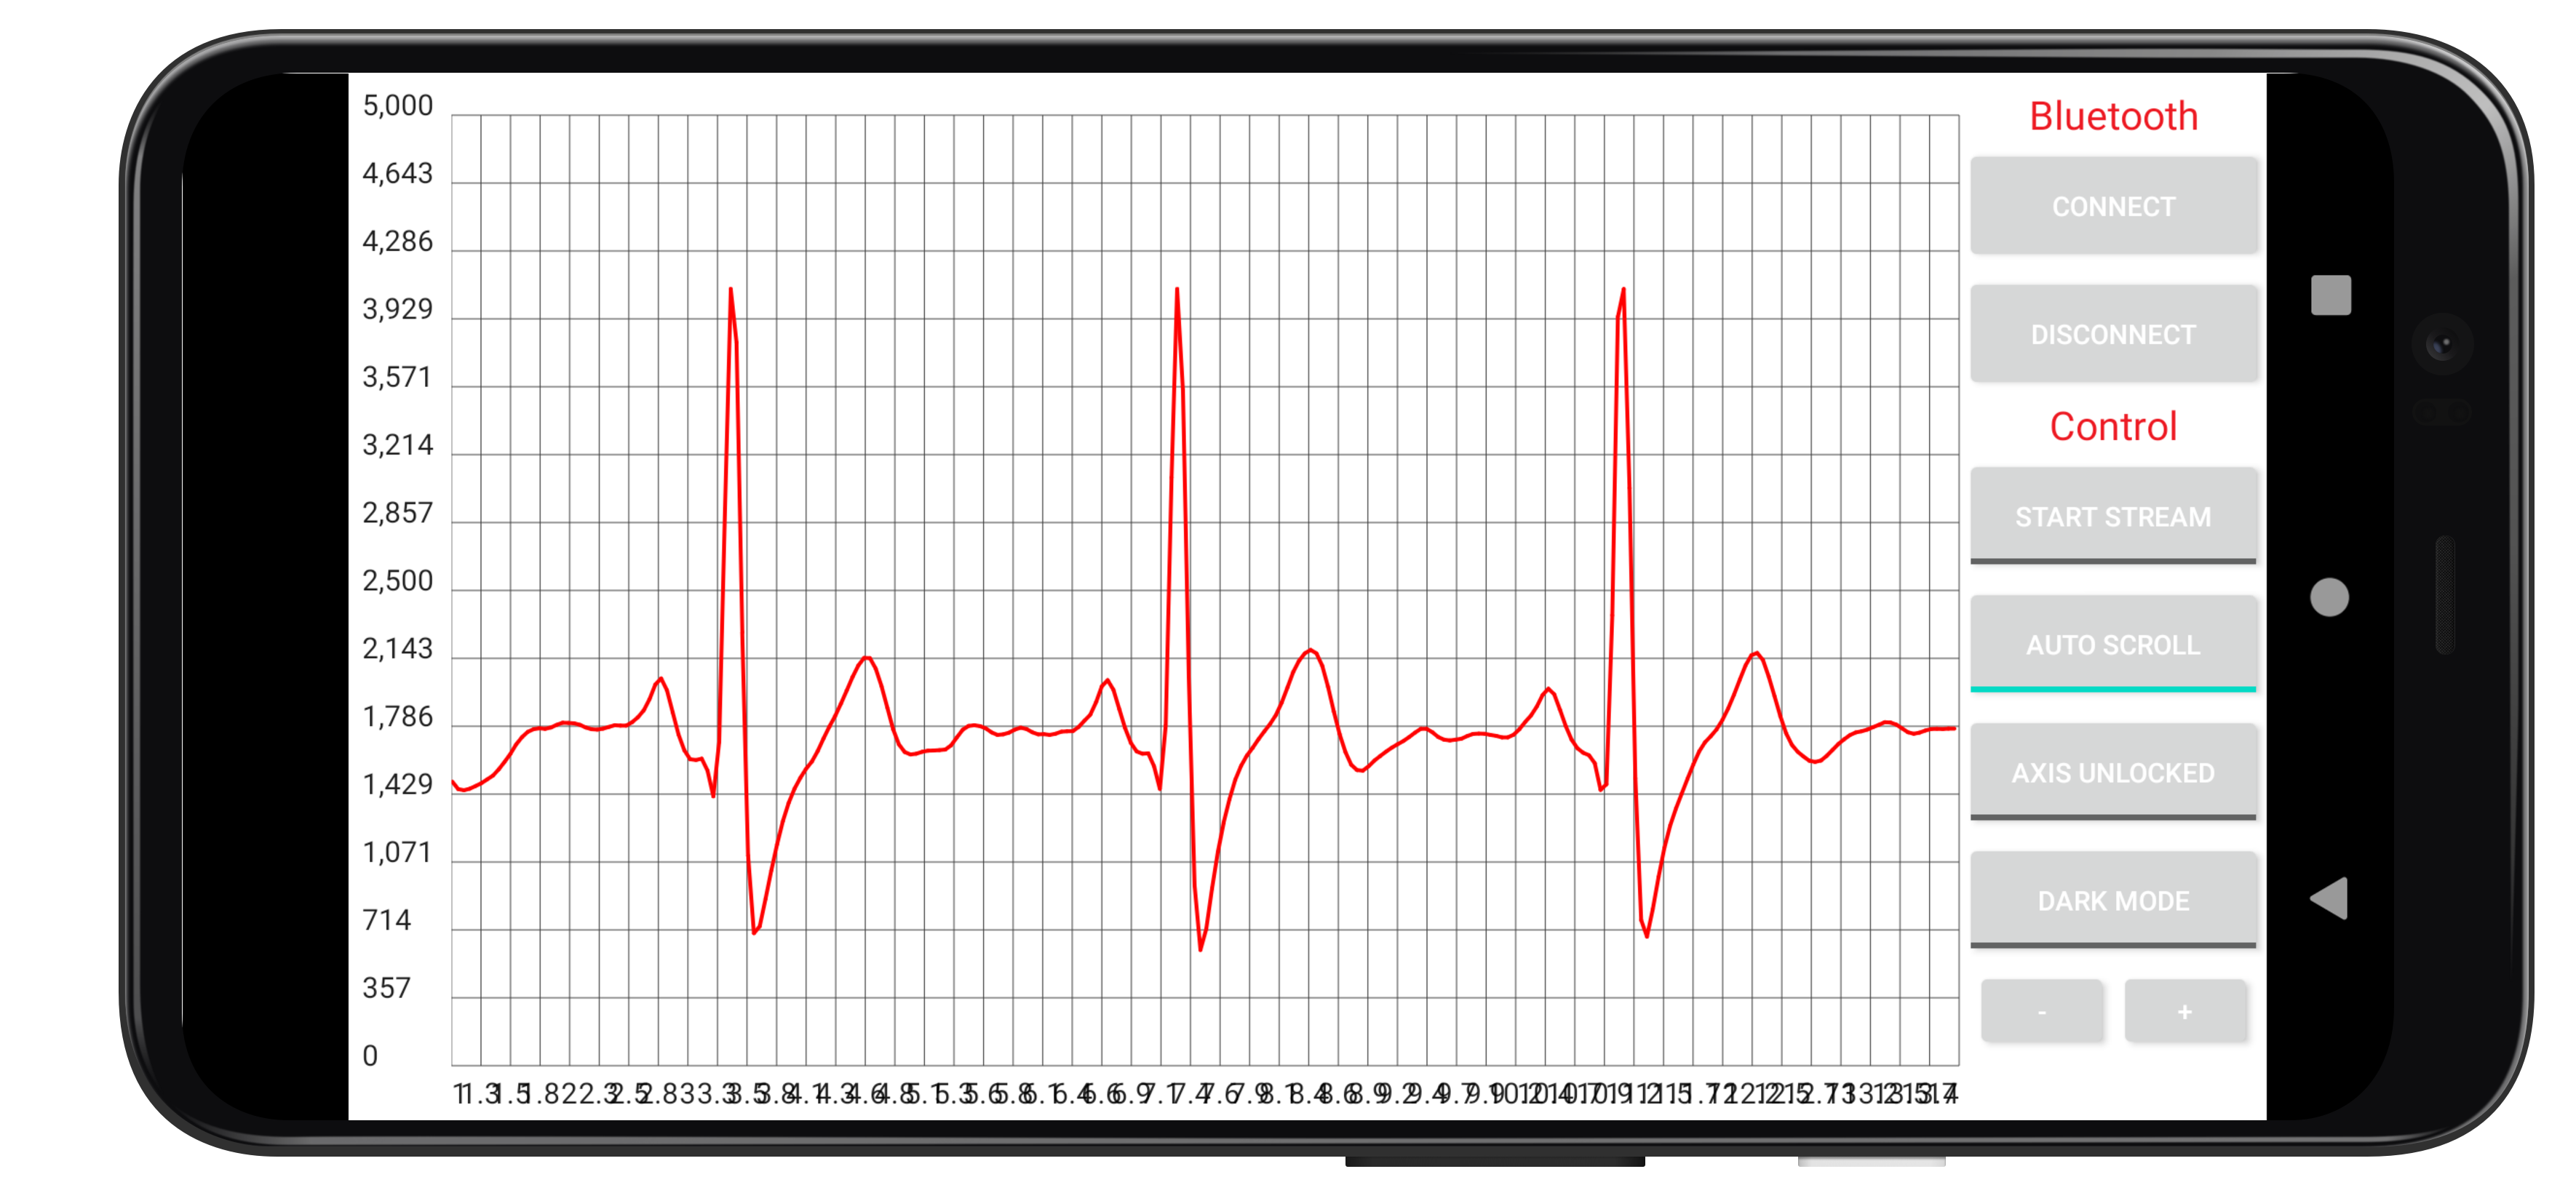
\includegraphics[width=\textwidth] {app_signal.png}
	\end{center}
	\caption{Signal Aktivität}
	\label{app_signal}
\end{figure}
\end{itemize}